\documentclass[12pt]{article}
\usepackage{sbc-template}
\usepackage{graphicx}
\usepackage{amsmath}
\usepackage{subfigure}
\usepackage{times,amsmath,epsfig}
\usepackage{graphicx,url}
  \makeatletter
  \newif\if@restonecol
  \makeatother
  \let\algorithm\relax
  \let\endalgorithm\relax
\usepackage[lined,algonl,ruled]{algorithm2e}
\usepackage{multirow}
\usepackage[brazil]{babel}
\usepackage[utf8]{inputenc}
\usepackage[pdftex]{hyperref}

\sloppy

\title{Algoritmos e Estruturas de Dados 3 \\ Trabalho Prático 6 \\
\huge{Auxiliar de Redação}}
\date{November 22, 1963}


\author{André Taiar Marinho Oliveira}


\address{Departamento de Ciência da Computação -- Universidade Federal de Minas Gerais (UFMG)
\email{taiar@dcc.ufmg.br}
\\
\\ Dezembro de 2010
}

\begin{document}

\maketitle

\begin{resumo}
\label{resumo}
Este relatório descreve a implementação de um sistema de auxílio à confecção de textos que, baseado em algumas premissas sobre más práticas para redação e estatísticas sobre palavras, frases, parágrafos e linhas, consegue indicar alguns pontos em que o texto pode ser melhorado. Foram sugeridas 3 situações em que o programa poderia indicar uma melhora das quais 2 foram implementadas. A primeira trabalha com estatísticas sobre os textos, indicando a ocorrência de parágrafos formados por apenas uma sentença, sentenças muito longas ou muito curtas (as análises também são feitas considerando e ignorando \textit{stop words} \footnote{Stop Words são palavras consideradas sem valor semântico para a análise de tópico de um texto (como artigos e preposições, por exemplo). \href{http://searchenginewatch.com/2156061}{Referência}.} ). A última trabalha com algumas expressões que são frequentemente utilizadas em uma língua mas teóricamente não existem e por isso devem ser evitadas nos textos.
\end{resumo}

\section{Introdução}
\label{introducao}

Uma cadeia de caracteres é uma sequência qualquer de elementos que podem ser representados como caracteres. Elas aparecem em várias áreas da computação: processamento de textos em linguagem natural, códigos, dicionários, sequenciamento de DNA em biologia computacional, representação de imagens por meio de bitmaps, entre outros. Neste trabalho, utilizamos a representação de um texto em linguagem natural como uma cadeia de caracteres e utilizamos algoritmos de processamento de cadeias de caracteres para reconhecer diversas informações pertinentes às análises que desejamos fazer.

Neste cenário, 2 tipos de algoritmos foram utilizados, um para cada situação a ser analisada. O primeiro foi um algoritmo baseado em autômato. Foi melhor abordar a modelagem dessa etapa com um autômato finito por se tratar de um parsing da cadeia de caracteres aonde diversos estados podem ser definidos, facilitando a análise com uma máquina de estados. O outro algoritmo, utilizado para resolver a etapa 3, foi um algoritmo de força bruta (que é o algoritmo mais simples para casamento de cadeias de caracteres). Mais detalhes sobre os algoritmos serão vistos na sessão \ref{solucao_proposta}.

Tanto as \textit{stop words} quanto as expressões e duas entradas de teste foram préviamente fornecidas pelos monitores para que pudéssemos rodar e testar o trabalho. Foi uma condição assumida que o texto não teria qualquer tipo de acentuação, portanto os arquivos de entrada, \textit{stop words} e expressões foram tratados e organizados para isso.

\section{Solução Proposta}
\label{solucao_proposta}

\subsection{Etapa 1}
Na Etapa 1 o programa deveria fornecer para cada parágrafo do texto:
\begin{enumerate}
  \item O número da linha no arquivo fonte aonde o parégrafo começa;
  \item o número de sentenças no parágrafo;
  \item para cada sentença, o número de palavras dela incluindo e não incluindo \textit{stop words}.	
\end{enumerate}

Respeitando as considerações feitas feitas na especificação acerca de marcação de parágrafos e palavras e sobre pontuação, foi elaborado um autômato que reconhece esse tipo de marcação no texto lendo a cadeia de caracteres um a um. Um exemplo do autômato pode ser visto na figura \ref{img:automato}.

\begin{figure}[ht!]
\centering
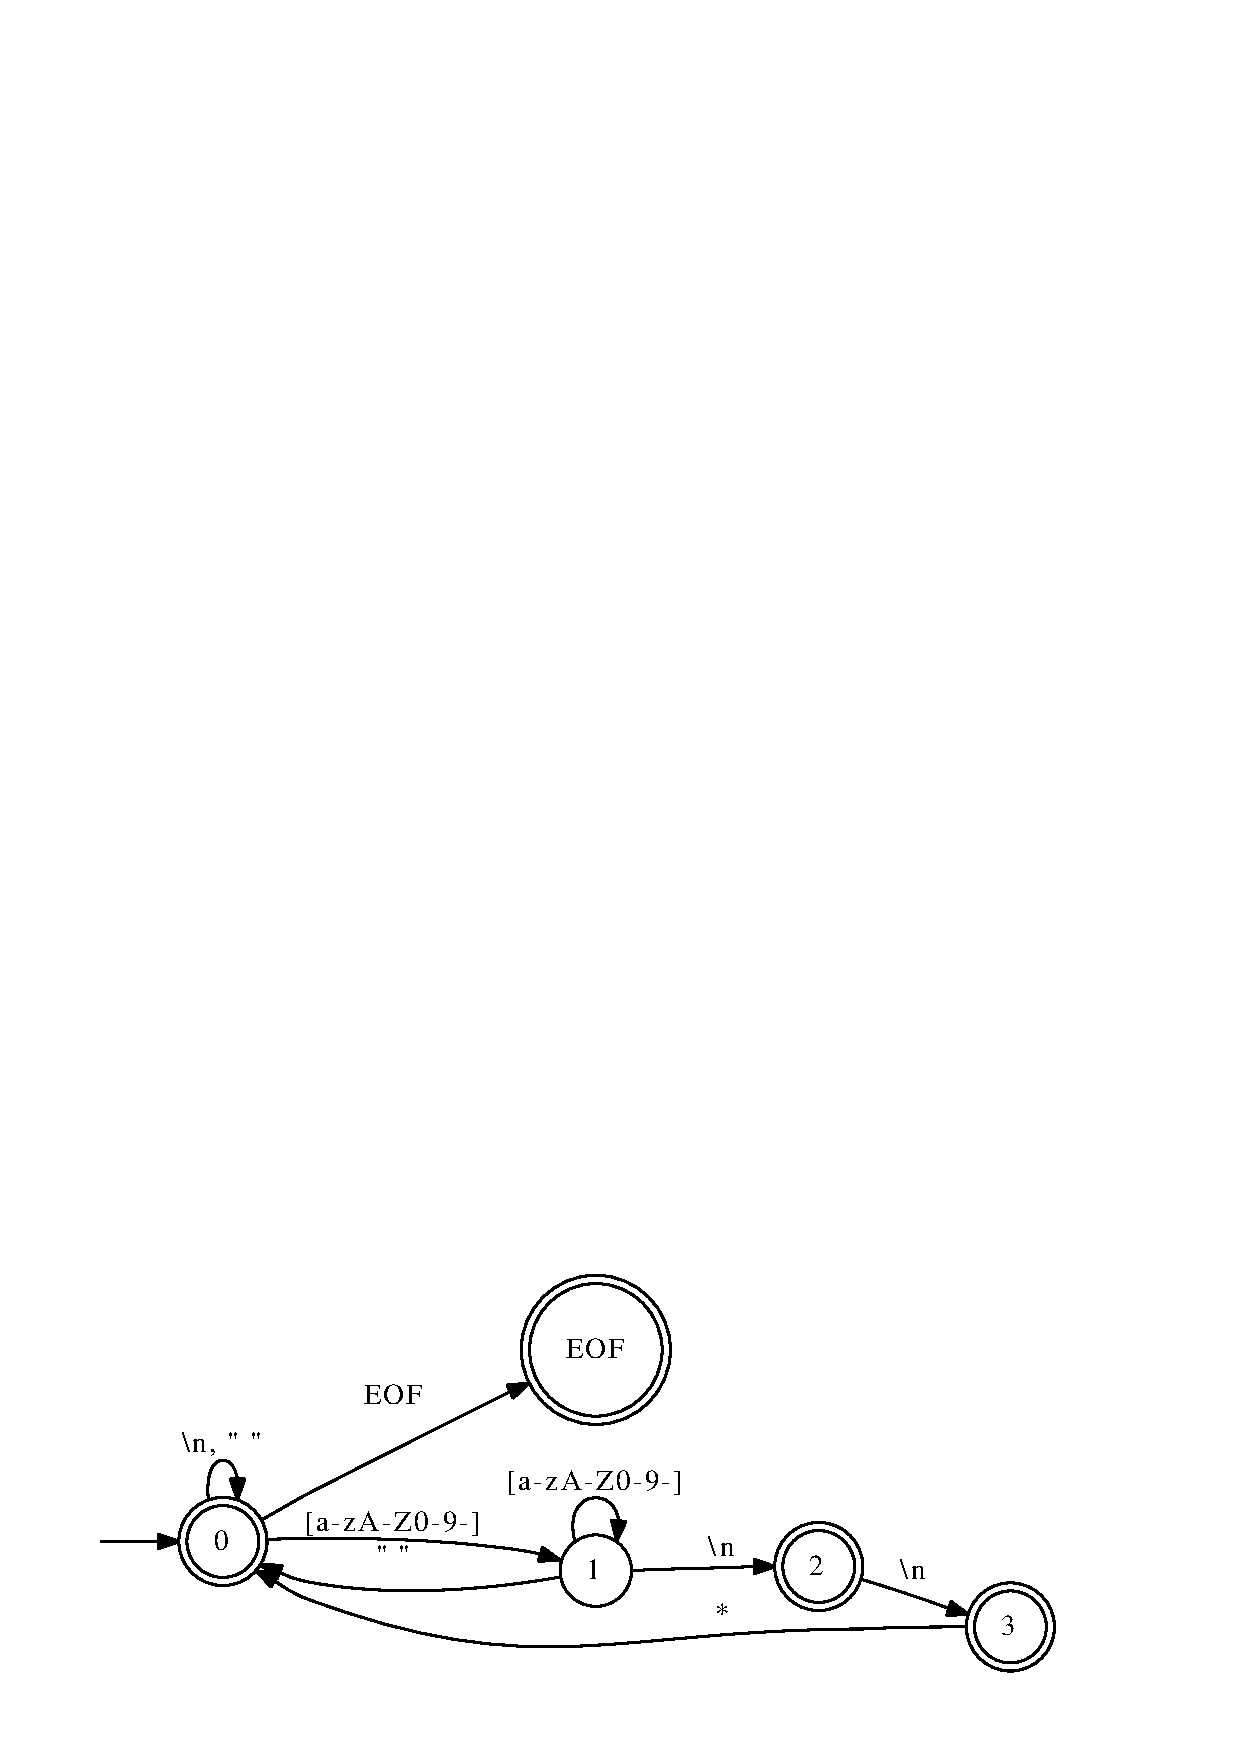
\includegraphics[width=10.0cm]{automato.pdf}
\label{img:automato}
\caption{Autômato de reconhecimento do texto}
\end{figure}

Em cada estado final ele retorna um sinal para que saibamos o que fazer com o valor capturado.
\begin{itemize}
  \item $1 \longrightarrow 0$ - casou uma palavra;
  \item $1 \longrightarrow 2$ - casou uma palavra;
  \item $2 \longrightarrow 3$ - casou um parágrafo;
  \item $3 \longrightarrow 0$ - é uma transição vazia ($\lambda$);
  \item $0 \longrightarrow EOF$ - retorna o fim do arquivo.
\end{itemize}

Dessa forma conseguimos interpretar o que está acontecendo com o texto à cada caractere que lemos da nossa cadeia, contabilizando semânticamente o que precisamos. As \textit{stop words} que devemos desconsiderar estão em um arquivo que é carregado na memória antes de varrermos o texto seguindo o autômato. Com as palavras em memória, vamos contabilizando as palavras que são e que não são \textit{stop words} à medida que o autômato casa os padrões. 

Como as \textit{stop words} estão ordenadas no arquivo que é passado, conseguimos determinar se uma palavra é ou não é relevante com uma ordem de complexidade menor do que $O(n)$. Assim, a complexidade total do algoritmo é $O(n)$; onde $n$ é o número de caracteres na cadeia de entrada (o número de caracteres do texto). Processando o texto como um autômato, precisamos apenas de uma passada para obter as informações que desejamos.

\subsection{Etapa 2}
Por ser opcional e pela falta de tempo de implementar a Etapa 2 do trabalho não foi implementada e não será discutida nem analisada no trabalho.

\subsection{Etapa 3}
Na Etapa 3 temos uma lista de expressões que não existem na língua portuguesa mas que costumam aparecer em alguns textos. Por isso, devemos localizá-las e indicar a linha em que ocorrem no texto. O algoritmo funciona carregando primeiramente a lista das expressões em memória. Em seguida, para cada uma das expressões, varremos o texto uma vez tentando casar a expressão com uma algoritmo de força bruta. Segue o pseudo-código do algoritmo:

\begin{algorithm}[h!]
\begin{footnotesize}
String $texto \longleftarrow$ cadeia de caracteres que vamos explorar\;
String $padrao\longleftarrow$ padrão que deve ser encontrado na cadeia de caracteres\;

\For{int $i=0$; $i < (length(texto) - length(padrao) + 1)$; $i+=1$}
{
  int $k = 1$\;
  int $j = 0$\;
  \While{$(j < m)$ \& $texto[k] == padrao[j]$}
  {
  	$j += 1;$
  	$k += 1;$
  	\If{$j == m$}
  	{
  		\Return "casou"\;
  	}
  }
}

Este algoritmo tem ordem $O(m * n)$ sendo $m$ o tamanho da cadeia de caracteres do texto e $n$ o tamanho da cadeia de caracteres do padrão a ser encontrado. Como fazemos isso para cada expressão em nossa lista de expressões, a complexidade total do algoritmo é $O(m * n * o)$; sendo $o$ o número de expressões que devemos checar.

\caption{Algoritmo de casamento de padrões por força bruta}
\end{footnotesize}
\end{algorithm}


\section{Código}

\subsection{Módulos}
O programa foi separado em três módulos:
\begin{itemize}
\item \textbf{Camadas:} define a estrutura da hierarquia de memória utilizada na simulação descrevendo as operações e estruturas de cada camada de memória. Faz a alocação e desalocação de todas essas estruturas.
\item \textbf{Simulação:} implementa a parte de simulação do trabalho operando sobre a estrutura de hierarquia de memória. Faz a contagem dos dados da simulação como hits, misses e tempos de execução. Além disso contém a implementação de todas as políticas de cache do trabalho.
\item \textbf{Principal:} faz a leitura inicial do arquivo de entrada e trabalha com os módulos Camadas e Simulação. Faz a contagem do tempo de execução das partes principais do programa para análise de complexidade.
\end{itemize}

\subsection{Entrada e saída}
\subsubsection{Linha de comando}
O trabalho não necessita de argumentos para funcionar. Todos os dados serão passados pela entrada principal. Porém, para facilitar a execução e os testes do trabalho, um arquivo pode ser passado como fonte para a entrada padrão da seguinte forma:

\begin{verbatim}
#: ./tp5 < /caminho/para/o/arquivo
\end{verbatim}

\subsubsection{Formato da entrada}
Em um mesmo arquivo podem existir vários casos de teste. Em cada um deles, uma hierarquia diferente de memória pode ser definida bem como a série de chamados a objetos em memória. O formato de cada teste é:
\begin{verbatim}
nCamdas vCam1 cCam1 polCam1 ... vCamn cCamn polCamn cCam0
nTestes
Data1 Time1
Data2 Time2
...
Datat Timet
\end{verbatim}$nCamdas$ - número de camadas adicionais na hierarquia; \\
$vCam_{i}$ - velocidade da camada de id \textit{i}; \\
$cCam_{i}$ - capacidade de armazenamento da camada de id \textit{i}; \\
$polCam_{i}$ - política de cache utilizada pela camada de id \textit{i}; \\
$cCam_{0}$ - capacidade de armazenameno da camada 0; \\
$nTestes$ - número de chamadas a dados que será feito na simulação; \\
$Data_{i}$ - referência ao dado de id \textit{i}; \\
$Time_{i}$ - tempo em que o dado de id \textit{i} foi requisitado.

\subsubsection{Formato da saída}
A saída do programa é retornada na saída padrão do sistema informando a taxa de HIT e MISS de cada camada da hierarquia além do tempo médio total da simulação.
\begin{verbatim}
Camada 1 => Cache Hit Ratio = tHit1; Cache Miss Ratio = tMiss1
Camada 2 => Cache Hit Ratio = tHit2; Cache Miss Ratio = tMiss2
...
Camada n => Cache Hit Ratio = tHitN; Cache Miss Ratio = tMissN
------
Tempo de resposta médio por requisição = tMedResp T
\end{verbatim}$tHit_{i}$ - taxa de HIT da camada de id \textit{i}; \\
$tMiss_{i}$ - taxa de MISS da camada de id \textit{i}; \\
$tMedResp$ - tempo médio de resposta de todas as requisições.

\subsection{Compilação}
O compilador utilizado neste trabalho foi o GCC (adotado como padrão para a disciplina) e 
o comando para compilar o programa através do GCC é:
\begin{verbatim}
  #: gcc -o tp5 tp5.c camadas.c camadas.h simulacao.c simulacao.h
\end{verbatim}
caso estejam todos os arquivos dentro do mesmo diretório.

Como pedido na especificação, foi feito um arquivo Makefile com o qual é possível compilar
o programa com o comando: 
\begin{verbatim}
  #: make main
\end{verbatim}

E podemos compilar e executar o programa com o comando:
\begin{verbatim}
  #: make run
\end{verbatim}
que fará, além da compilação, com que o programa execute com uma entrada pequena.

\section{Avaliação Experimental}
\label{avaliacao_experimental}

\subsection{Qual o custo computacional da substituição de um objeto? Qual o custo em memória?}

\begin{table}[htb]
\centering
\caption{Custo computacional e Custo em memória da substituição de um objeto}
\begin{tabular}{|c|c|c|}
\hline  & Custo Computacional & Custo em Memória \\ 
\hline lru & $O(n)$ & $O(n)$ \\ 
\hline lfu & $O(n)$ & $O(n)$ \\ 
\hline mru & $O(n)$ & $O(n)$ \\ 
\hline fifo & $O(n)$ & $O(n)$ \\ 
\hline 
\end{tabular}
\end{table}

O custo computacional para a substituição de todas as políticas é $O(n)$, com n
sendo a capacidade de armazenamento da camada pois em todas as políticas conseguimos 
identificar o elemento que deverá deixar a memória com apenas um leitura completa do 
vetor.

O mesmo se aplica ao custo em memória que será sempre em função da capacidade
máxima de armazenamento da camada.

\subsection{Qual o custo total da execução da simulação? E o custo em memória?}

Tomando como pior caso para a análise quando o miss acontece em todas as
camadas, para cada um dos testes $t_{i}$ vamos passar por todas as camadas
$c_{j}$ e percorrer toda a sua memória $m_{j}$ da camada tornando o algoritmo
$O(t*c*m)$. O custo em memória para o mesmo cenário é $O(c*m)$ pois não sofre
qualquer alteração com o aumento do número de testes uma vez que eles não são
armazenados na memória.

\subsection{Simulações individuais para cada política comparadas com o custo
computacional do trabalho}

\subsection{Qual o custo computacional da substituição de um objeto? Qual o custo em memória?}
Plotar

%\begin{figure}[ht!]
%\centering
%\includegraphics[width=3.5cm,height=2.8cm]{avaliacoes/testes.png}
%\label{img:resss}
%\caption{Gráfico dos tempos de execução}
%\end{figure}

\section{Conclusões}
\label{conclusao}

Por falta de tempo para implementar deixo aqui algumas idéias que fariam análises mais interessantes sobre o assunto e tornaria este trabalho mais proveitoso:
\begin{itemize}
  \item Uma boa idéia seria uti
\end{itemize}

\end{document}
